\item A qué valor de presión de aire se debe inflar un neumático (fig. \ref{fig:neumatico}) de un auto de carrera en boxes teniendo en cuenta que cuando esté en carrera la temperatura del neumático será de $T_n$ y la presión optima deberá ser de $P_{opt}$? Considerar la temperatura del neumático frio en boxes de 20 $^\circ$C y el volumen del mismo es de $V_n$. El aumento de volumen del neumático de frio a caliente es del $20\%$. Suponga que la presión atmosférica es de 100 KPa.

%% Esto son datos centrados
\begin{center}
$T_n = 60 \, ^\circ C \qquad P_{opt} = 40\,\text{psi} \qquad V_n =  0.025\,\text{m}^3$
\end{center}
%% Esto es una figura

\begin{figure}[h]
\centering
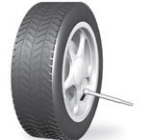
\includegraphics[width=0.2\textwidth]{neumatico.png}
\caption{Neumático}
\label{fig:neumatico}
\end{figure}
